\documentclass{beamer}
\usetheme{default}

\usepackage{amsmath, amssymb, amsfonts}
\usepackage{tikz}
\usetikzlibrary{arrows.meta, calc, positioning}

\title{Hyperplane Arrangements and Combinatorial Complexity}
\author{Siddharth Krishna}
\date{November 2025}

\begin{document}

\frame{\titlepage}

%---------------------------------------------------------
\begin{frame}{What is a Hyperplane Arrangement?}
A \emph{hyperplane arrangement} $\mathcal A$ in $\mathbb{R}^d$ is a finite set of affine hyperplanes:

\[
\mathcal A = \{ H_1,\dots, H_n \}, \qquad
H_i = \{x \in \mathbb R^d : w_i \cdot x + b_i = 0\}.
\]

\begin{center}
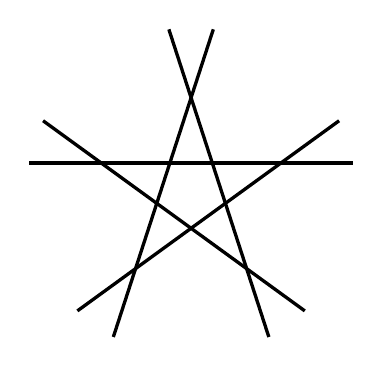
\begin{tikzpicture}[scale=1]
  % Define the 5 vertices of a regular pentagon (for the star)
  \foreach \k in {0,...,4} {
    \path ({90+72*\k}:1.2) coordinate (P\k);
  }

  % Draw 5 lines, each extending the edges of the 5-point star
  \foreach \k in {0,...,4} {
    \pgfmathtruncatemacro{\kk}{mod(\k+2,5)} % connect every second vertex (star)
    % Extend the segment beyond both ends to make a full "hyperplane"
    \draw[very thick]
      ($(P\k)!-0.4!(P\kk)$) -- ($(P\k)!1.4!(P\kk)$);
  }
\end{tikzpicture}
\end{center}

\begin{itemize}
  \item Even a few hyperplanes create interesting region structure.
  \item These regions encode combinatorial data.
\end{itemize}
\end{frame}

%---------------------------------------------------------
\begin{frame}{Examples of Arrangements}
\begin{columns}
\column{0.5\textwidth}
\begin{center}
\textbf{Two lines = 4 regions}
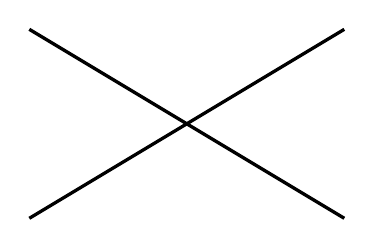
\begin{tikzpicture}[scale=1.0]
  \draw[very thick] (-2,-1.2) -- (2,1.2);
  \draw[very thick] (-2,1.2) -- (2,-1.2);
\end{tikzpicture}
\end{center}

\column{0.5\textwidth}
\begin{center}
\textbf{Three lines = 7 regions}
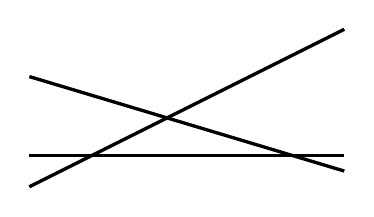
\begin{tikzpicture}[scale=1.0]
  % three lines in general position (no triple intersection)
  \draw[very thick] (-2,0) -- (2,0);           % horizontal
  \draw[very thick] (-2,-0.4) -- (2,1.6);      % slightly up-sloping
  \draw[very thick] (-2,1.0) -- (2,-0.2);      % down-sloping, shifted
\end{tikzpicture}
\end{center}
\end{columns}
\end{frame}

%---------------------------------------------------------
\begin{frame}{Sign Patterns}
For hyperplanes $H_i: w_i \cdot x + b_i = 0$, define
\[
\sigma(x)=\bigl(\operatorname{sign}(w_1\cdot x+b_1),\dots,\operatorname{sign}(w_n\cdot x+b_n)\bigr).
\]

\begin{block}{Key fact}
Two points lie in the same region $\iff$ they have the same sign pattern.
\end{block}

\pause

\begin{itemize}
\item Regions correspond to consistent choices of $+$ and $-$ for each hyperplane.
\end{itemize}
\end{frame}

%---------------------------------------------------------
\begin{frame}{Intersection Poset}
The \emph{intersection poset} $L(\mathcal{A})$ contains all intersections of hyperplanes, ordered by reverse inclusion.

\medskip
\begin{center}
\textbf{Example: Two lines}
\end{center}

\begin{columns}[c]

% ---- LEFT COLUMN: Geometry picture ----
\column{0.45\textwidth}
\begin{center}
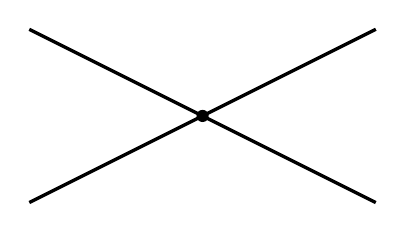
\begin{tikzpicture}[scale=1.1, thick]
  % Two nonparallel lines
  \draw[very thick] (-2,-1) -- (2,1);
  \draw[very thick] (-2,1) -- (2,-1);

  % intersection point
  \fill (0,0) circle (2pt);
\end{tikzpicture}
\end{center}

% ---- RIGHT COLUMN: Hasse diagram ----
\column{0.55\textwidth}
\begin{center}
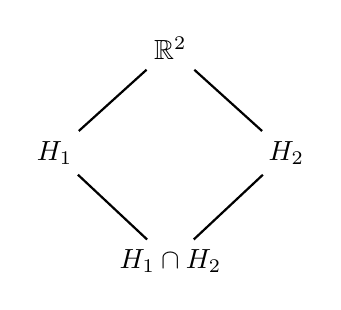
\begin{tikzpicture}[node distance=1.1cm, thick]
  \node (top) {$\mathbb{R}^2$};
  \node (L1) [below left=of top] {$H_1$};
  \node (L2) [below right=of top] {$H_2$};
  \node (pt) [below=of $(L1)!0.5!(L2)$] {$H_1 \cap H_2$};

  \draw (top) -- (L1);
  \draw (top) -- (L2);
  \draw (L1) -- (pt);
  \draw (L2) -- (pt);
\end{tikzpicture}
\end{center}
\end{columns}
\end{frame}

%---------------------------------------------------------
\begin{frame}{Characteristic Polynomial}
Defined by
\[
\chi_{\mathcal{A}}(t)=
\sum_{X\in L(\mathcal{A})} \mu(\mathbb{R}^d,X)\, t^{\dim X}.
\]

\pause

Example: Two nonparallel lines in $\mathbb{R}^2$:
\[
\chi(t) = t^2 - 2t +1.
\]

\pause

\[
\chi(-1) = 4 = \text{number of regions.}
\]
\end{frame}

%---------------------------------------------------------
\begin{frame}{Zaslavsky's Theorem}
\[
r(\mathcal{A}) = (-1)^{\text{rank}(\mathcal A)}\, \chi_{\mathcal{A}}(-1)
\]
\[
b(\mathcal{A}) = (-1)^{\text{rank}(\mathcal A)}\, \chi_{\mathcal{A}}(1)
\]

\pause

\begin{block}{Idea of proof}
Deleting a hyperplane or restricting to it gives a recurrence for region counts.
The characteristic polynomial satisfies the same recurrence.  
Conclude by induction.
\end{block}
\end{frame}

%---------------------------------------------------------
\begin{frame}{Deletion--Restriction Diagram}
\begin{center}
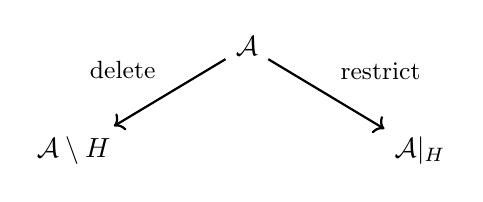
\begin{tikzpicture}[scale=1.1, thick]
  \node (A) at (0,0) {$\mathcal{A}$};
  \node (Ad) at (-2,-1.2) {$\mathcal{A}\setminus H$};
  \node (Ar) at (2,-1.2) {$\mathcal{A}|_H$};

  \draw[->] (A) -- node[above left=2pt] {\small delete} (Ad);
  \draw[->] (A) -- node[above right=2pt] {\small restrict} (Ar);
\end{tikzpicture}
\end{center}

\[
r(\mathcal{A}) = r(\mathcal{A}\setminus H) + r(\mathcal{A}|_H)
\]
\end{frame}

%---------------------------------------------------------
\begin{frame}{Face Poset}

\begin{center}
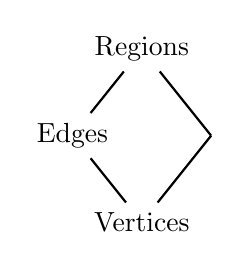
\begin{tikzpicture}[scale=1.1, thick]
  \node (R) at (0,1.4) {Regions};
  \node (E1) at (-0.8,0.4) {Edges};
  \node (E2) at (0.8,0.4) {};
  \node (V) at (0,-0.6) {Vertices};

  \draw (R) -- (E1);
  \draw (R) -- (0.8,0.4);
  \draw (E1) -- (V);
  \draw (0.8,0.4) -- (V);
\end{tikzpicture}
\end{center}

\begin{itemize}
  \item Faces are ordered by \emph{closure inclusion}:  
        $F \le G \iff \overline{F} \subseteq \overline{G}$.
  \item Maximal elements are the regions.
  \item Encodes adjacency and how the stratification fits together.
\end{itemize}

\end{frame}

%---------------------------------------------------------
\begin{frame}{Sign Vectors and Adjacency}
\[
\sigma(x)\in\{-,0,+\}^n
\]

\begin{itemize}
  \item Zero entries: point lies on a hyperplane.
  \item No zeros: interior of a region.
  \item Adjacent regions differ in exactly one sign coordinate.
\end{itemize}

\pause

This is the oriented structure of the arrangement.
\end{frame}

%---------------------------------------------------------
\begin{frame}{ReLU = Hyperplane Arrangement}

A ReLU unit computes:
\[
\operatorname{ReLU}(w \cdot x + b) = \max(0,\, w \cdot x + b).
\]

Its activation boundary is the hyperplane
\[
w \cdot x + b = 0.
\]

A layer with $n$ ReLU units in $\mathbb R^d$ produces $n$ such hyperplanes.

\begin{center}
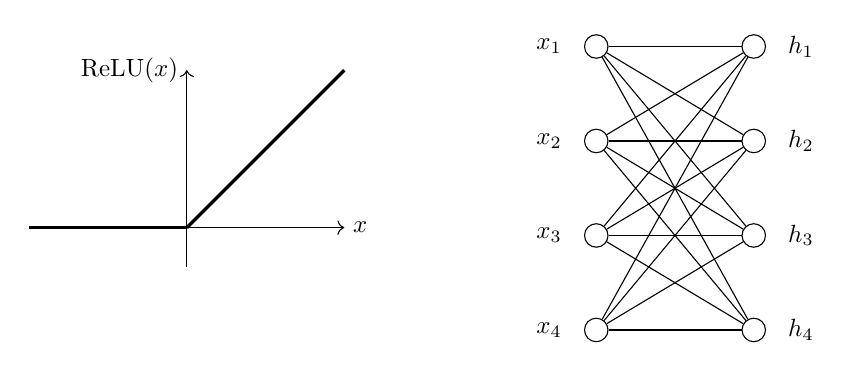
\begin{tikzpicture}[scale=1, every node/.style={scale=0.9}]

% -----------------------
% RIGHT: MLP diagram (vertical, pointing downward)
% -----------------------

\begin{scope}[shift={(2, 0.5)}]

  % Input nodes (top)
  \foreach \i in {1,...,4} {
    \node[circle, draw, fill=white] (x\i) at (0,-1.2*\i) {};
    \node at (-0.6,-1.2*\i) {$x_{\i}$};
  }

  % Output / ReLU nodes (below inputs)
  \foreach \j in {1,...,4} {
    \node[circle, draw, fill=white] (h\j) at (2,-1.2*\j) {};
    \node at (2.6,-1.2*\j) {$h_{\j}$};
  }

  % Fully connected edges
  \foreach \i in {1,...,4} {
    \foreach \j in {1,...,4} {
      \draw (x\i) -- (h\j);
    }
  }

\end{scope}

% -----------------------
% LEFT: Graph of ReLU
% -----------------------

\begin{scope}[shift={(-3.2,-3)}]
  % axes
  \draw[->] (-2,0) -- (2,0) node[right] {$x$};
  \draw[->] (0,-0.5) -- (0,2) node[left] {$\operatorname{ReLU}(x)$};

  % ReLU graph
  \draw[very thick] (-2,0) -- (0,0);
  \draw[very thick] (0,0) -- (2,2);
\end{scope}

\end{tikzpicture}
\end{center}

\end{frame}

%---------------------------------------------------------
\begin{frame}{Linear Regions of a ReLU Layer}
\begin{itemize}
  \item On each region, all signs are fixed.
  \item Therefore the layer is \emph{linear} on each region.
  \item Regions = linear pieces.
\end{itemize}

\[
\#\text{linear pieces} = r(\mathcal{A}) = (-1)^d \chi_{\mathcal{A}}(-1).
\]
\end{frame}

%---------------------------------------------------------
\begin{frame}{Fragility and Decision Boundaries}
\begin{itemize}
  \item Near intersections of several hyperplanes, even tiny perturbations can move an input into a different region.
  \item Crossing multiple boundaries flips multiple ReLUs at once, changing the affine function applied.
  \item This offers a geometric explanation for adversarial sensitivity.
\end{itemize}

\begin{center}
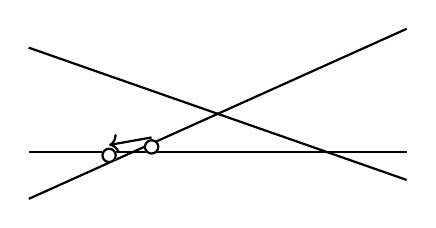
\begin{tikzpicture}[scale=1.2, thick]

  % --- hyperplanes (3 lines in general position) ---
  \draw (-2,0) -- (2,0);
  \draw (-2,1.1) -- (2,-0.3);
  \draw (-2,-0.5) -- (2,1.3);

  % --- point near intersection ---
  \filldraw[white, fill=white] (-0.7,0.05) circle (2pt);
  \draw (-0.7,0.05) circle (2pt);

  % --- perturbed point ---
  \filldraw[white, fill=white] (-1.15,-0.04) circle (2pt);
  \draw (-1.15,-0.04) circle (2pt);
  
  % --- perturbation arrow ---
  \draw[->, thick] (-0.7,0.05+0.1) -- (-1.15,-0.03+0.1);

\end{tikzpicture}
\end{center}

\end{frame}

%---------------------------------------------------------
\begin{frame}{Conclusion}
\begin{itemize}
  \item Hyperplane arrangements provide a clean combinatorial description of region structure.
  \item Zaslavsky’s theorem turns region counting into a poset computation.
  \item ReLU networks naturally inherit this structure: regions correspond to linear behaviors of the layer.
\end{itemize}
\end{frame}

%---------------------------------------------------------
\begin{frame}{References}
\footnotesize
\begin{thebibliography}{9}

\bibitem{ChenWang}
A.~Chen and A.~Wang,
\emph{Intersection Posets, Characteristic Polynomials, and Regions},
MIT PRIMES Conference (2017).
\url{https://math.mit.edu/research/highschool/primes/materials/2017/conf/Chen-Wang.pdf}

\end{thebibliography}
\end{frame}

\end{document}